\section{Risultati ottenuti}
Il confronto delle differenti topologie di rete con un numero crescente di layer nascosti ha prodotto i risultati riportati in Tabella \ref{tab:topology}.
\begin{table}
	\centering
	\caption{Tabella riportante il valore medio di AUC in \textit{3-fold cross validation} per le differenti topologie di rete.}
	\begin{tabular}{c|c}
		\label{tab:topology}
		\textbf{Numero di layer nascosti} & \textbf{AUC media} \\
		3 & 0.831 \\ 
		4 & 0.826 \\ 
		5 & 0.828 \\
	\end{tabular}
\end{table}

Per quanto concerne il processo di ottimizzazione degli iperparametri, i valori di \textit{best seen} per ogni possibile input della rete sono riportati in Tabella \ref{tab:bestseen}. 
In Figura \ref{subfig:best-seen} è riportata l'evoluzione del valore di \textit{best seen} ad ogni \textit{step} del processo di ottimizzazione per tutte le possibili strategie di input.
In aggiunta, in Figura \ref{subfig:auc-iteration} è riportato il valore di AUC media ottenuto con l'\textit{i}-esima configurazione durante il processo di ottimizzazione.
\newpage
\begin{figure}[!h]
	\begin{tabular}{cc}
		\subfloat[\label{subfig:best-seen}Sull'asse delle \textit{x} è riportata l'iterazione del processo di ottimizzazione, mentre sull'asse delle \textit{y} il valore di AUC media massimo ottenuto fino a quello \textit{step}.]{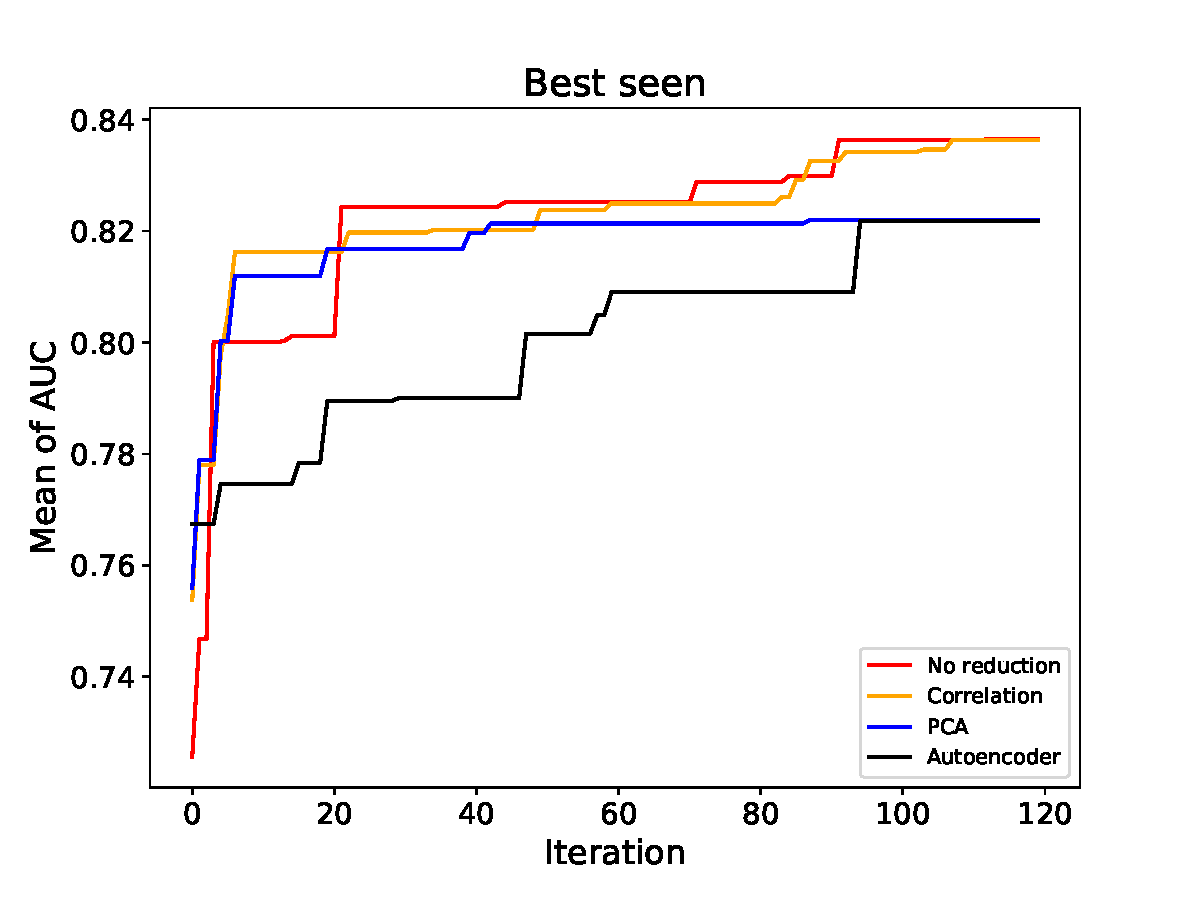
\includegraphics[width = .5\textwidth]{../images/pdf/best-seen}} &
		\subfloat[\label{subfig:auc-iteration}Sull'asse delle \textit{x} si riporta l'\textit{i}-esima iterazione del processo di ottimizzazione, sull'asse delle \textit{y} si riporta il relativo valore di AUC media ottenuto in quello \textit{step}.]{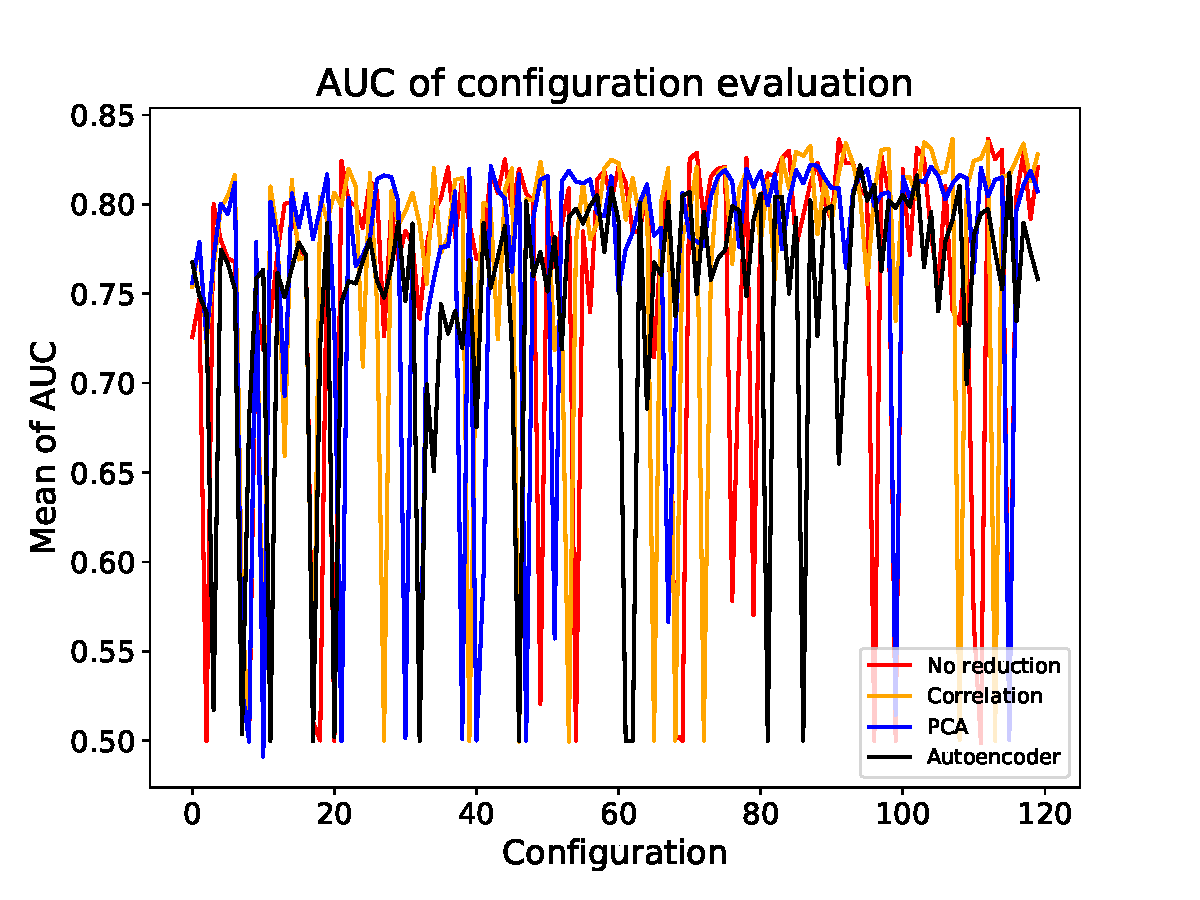
\includegraphics[width = .5\textwidth]{../images/pdf/AUC-iteration}} 
	\end{tabular}
	\caption{In Figura \ref{subfig:best-seen} è riportata l'evoluzione del \textit{best seen} durante il processo di ottimizzazione, mentre in Figura \ref{subfig:auc-iteration} è presente il valore di AUC media all'\textit{i}-esima iterazione.}
	\label{fig:HPO}
\end{figure}
\begin{table}[!b]
	\centering
	\caption{Tabella riportante per ogni tecnica di feature reduction il valore di AUC media sulle 12 label della configurazione ottima di iperparametri, individuata da un processo di ottimizzazione SMBO.}
	\begin{tabular}{c|c}
		\label{tab:bestseen}
		\textbf{Tecnica utilizzata} & \textbf{AUC media} \\
		Nessuna & 0.837 \\ 
		Correlazione & 0.836 \\ 
		PCA & 0.822 \\ 
		Encoder & 0.821 \\ 
	\end{tabular}
\end{table}
\begin{table}[!h]
	\centering
	\caption{Per ogni tecnica di FR (Feature Reduction) sono riportate le configurazioni ottime degli iperparametri individuate del processo di ottimizzazione.}
	\begin{tabular}{|c|c|c|c|c|c|}
		\label{tab:hporesult}
		\textbf{Tecnica di FR} & \textbf{Attivazione} & \textbf{Batch Size} & \textbf{Dropout} & \textbf{L2} & \textbf{Weight} \\
		Nessuna & relu & $128$ & $0.26$ & $0$ & $1.06$ \\ 
		Correlazione & relu & $256$ & $0.36$ & $0.0001$ & $0.82$ \\ 
		PCA & relu & $512$ & $0.2$ & $0.0322$ & $11.75$ \\ 
		Autoencoder & relu & $256$ & $0.55$ & $0.0004$ & $23.65$ \\ 
	\end{tabular} 
\end{table}
La Tabella \ref{tab:hporesult} riporta le configurazioni ottimali degli iperparametri individuate dal processo di ottimizzazione per i differenti input forniti; nella Tabella è inoltre riportato il valore di AUC associato alla configurazione.
\begin{figure}
	\begin{tabular}{cc}
		\subfloat[\label{subfig:roc}ROC rispettive alle dodici label, sono state calcolate usando il modello con la strategia di feature reduction scelta e relativa configurazione di iperparametri ottimi.]{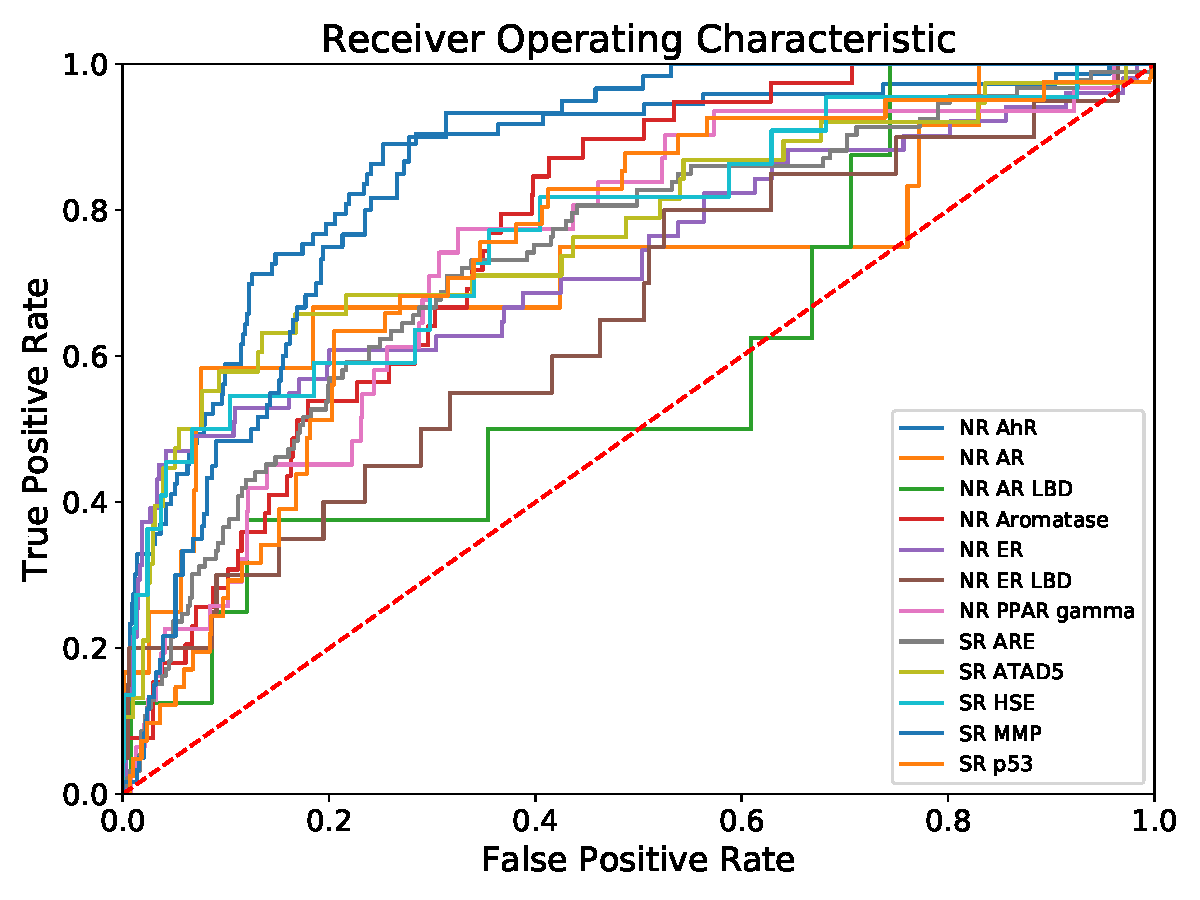
\includegraphics[width = .5\textwidth]{../images/pdf/ROC}} &
		\subfloat[\label{subfig:pr}Raffigurazione di come all'evolvere del \%TP variano i valori di precision e recall del modello.]{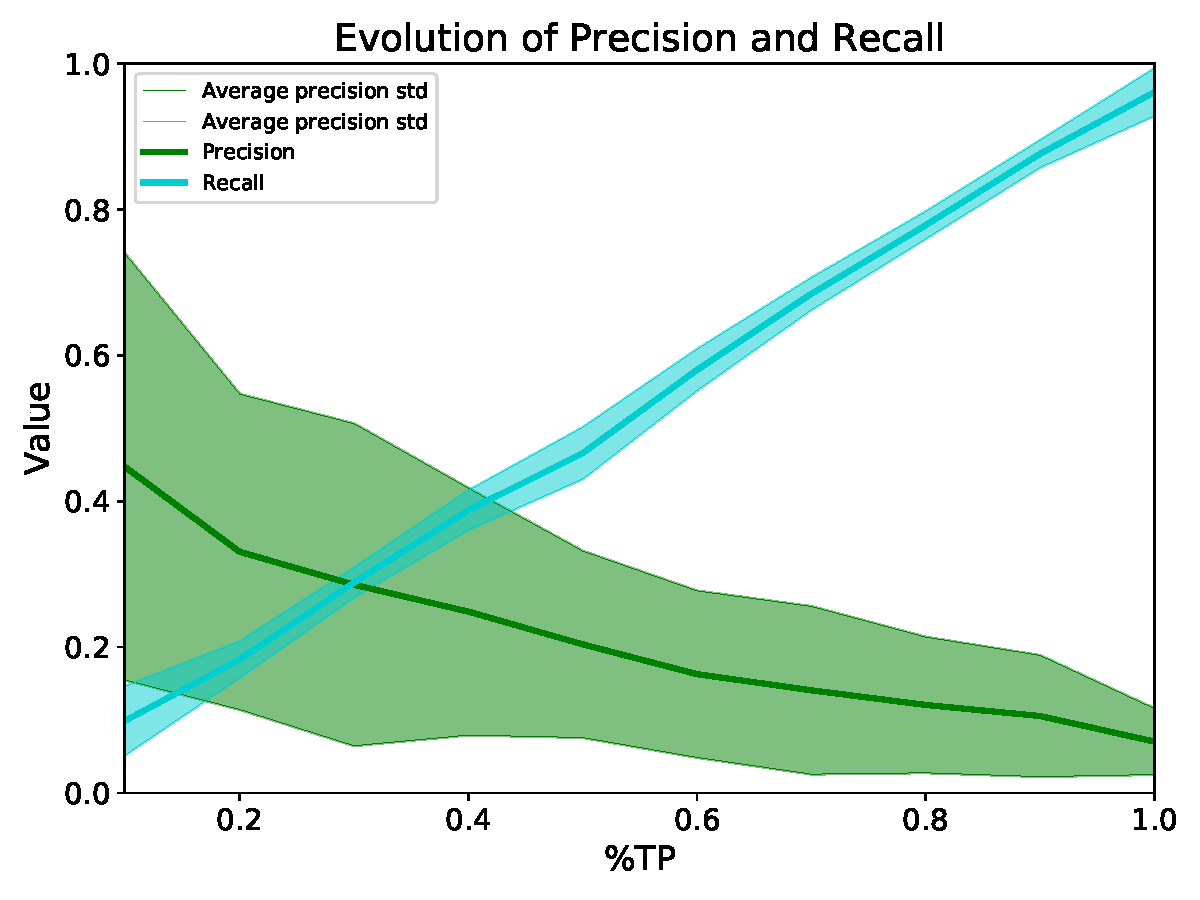
\includegraphics[width = .5\textwidth]{../images/pdf/pr_evolution}} 
	\end{tabular}
	\caption{In Figura \ref{subfig:roc} si mostrano le ROC relative alle 12 label, mentre in Figura \ref{subfig:pr} l'evoluzione di precision e recall all'aumentare del \%TP richiesto.}
	\label{fig:roc-pr}
\end{figure} 

Infine, si riportano i risultati riguardanti le analisi sul modello considerato ottimale, ovvero quello con la strategia scelta di feature reduction e i relativi iperparametri ottimi.
In Figura \ref{subfig:roc} sono rappresentate le curve ROC per ogni label, mentre in Figura \ref{subfig:pr} si mostra come all'evolvere della \%TP desiderata, evolvono la recall e precision del modello.
Per concludere, in Figura \ref{fig:comparison} sono presentate le performance del modello proposto in questo lavoro e degli altri elencati nel \textit{paper} di riferimento \cite{mayr2016deeptox}; il confronto avviene sui valori di AUC per ognuna delle 12 label, per media delle AUC su tutte le label (AVG) e per media delle AUC delle label inerenti ai due macro-gruppi SR, NR.
\begin{figure}[!t]
	\centering
	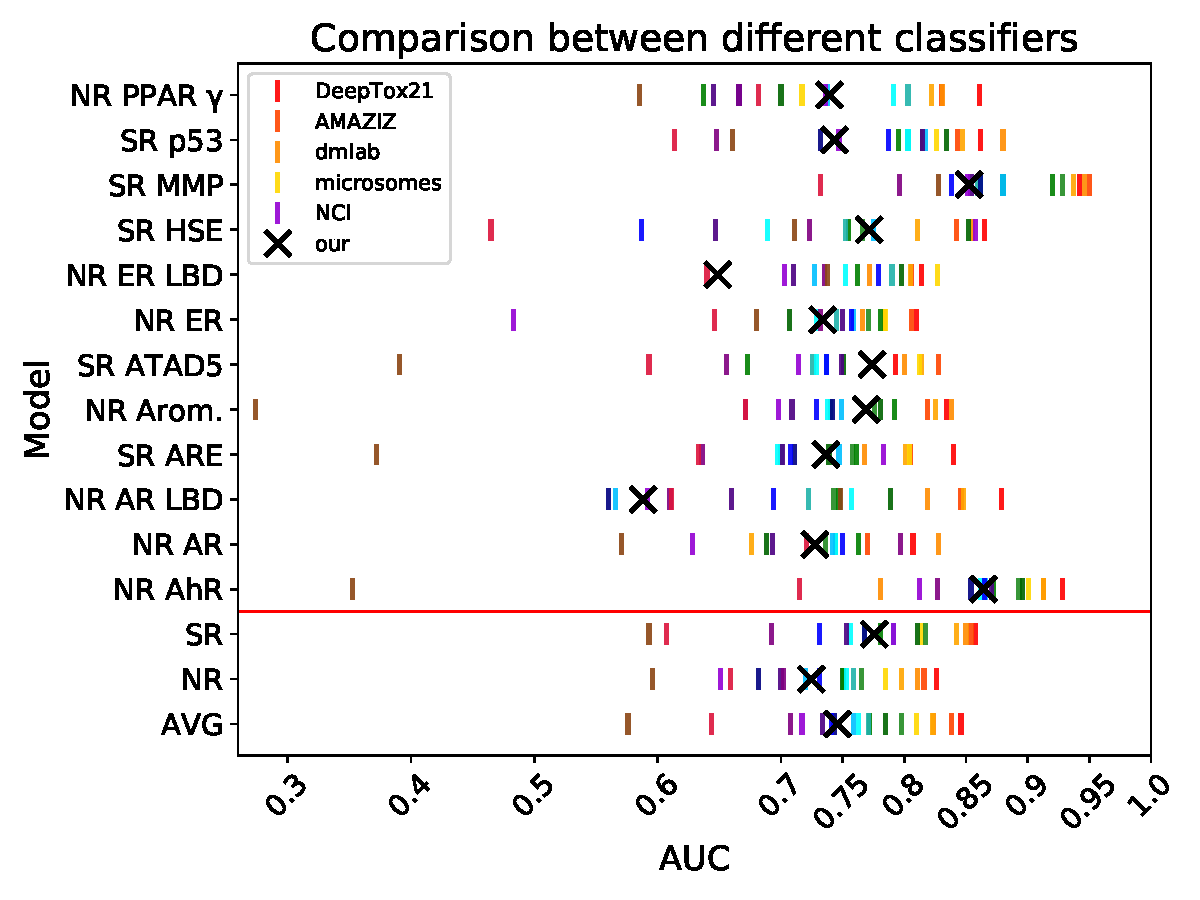
\includegraphics[width=0.9\linewidth]{../images/pdf/comparison}
	\caption{Confronto di vari modelli rispetto alle AUC (o media di AUC). Le linee rappresentano i modelli elencati nel lavoro di riferimento \cite{mayr2016deeptox}, mentre con la 'X' si indica il modello presentato in questo lavoro. Oltre alle AUC rispettive delle 12 label, sotto la linea rossa sono presentati i valori medi su tutte le label (AVG), sulle label relative agli SR e alle NR. Sono riportati in legenda (oltre al modello di questo lavoro) i modelli che sono risultati tra i primi due per quanto riguarda una label o una delle medie.}
	\label{fig:comparison}
\end{figure}